\chapter{Progettazione Concettuale/Logica}


%fare introduzione capitolo...


\section{Modellazione NoAM $\to$ NoSQL abstract model}
La metodologia NoAM é composta da:
\begin{itemize}
    \item Modellazione Concettuale e design degli Aggregati
    \item Partizionamento degli Aggregati e modellazione NoSQL
    \item Implementazione
\end{itemize}

\subsection{Modellazione Concettuale e design degli Aggregati}
Riguarda la vera e propria progettazione del modello di dominio, e comporta l'identificazione
delle diverse classi di aggregati necessari in un'applicazione.
Sono possibili diversi approcci per identificare classi di aggregati per una particolare applicazione.
L'approccio Domain-Driven Design(\emph{DDD}), attraverso il quale viene generato un diagramma UML delle classi,
é guidato dai casi d'uso, ovvero dai requisiti funzionali, e da esigenze di scalabilitá e coerenza all'interno dell'aggregato.
Si procede nel modo seguente:
\begin{itemize}
    \item I dati persistenti di un'applicazione sono modellati in termini di entitá, oggetti di valore e
    relazioni.
    Un'entitá é un oggetto persistente che ha un'esistenza indipendente ed é caratterizzata da un'identificatore
    univoco, mentre un oggetto di valore é caratterizzato appunto da un suo valore senza un proprio identificatore
    \item Entitá e oggetti di valore vengono raggruppati in \emph{aggregati}.
    Un aggregato ha un'entitá come radice e puó contenere molti oggetti di valore.
\end{itemize}
A causa delle loro caratteristiche, la progettazione degli aggregati comporta un compromesso per quanto riguarda
la loro granularitá. infatti:
\begin{itemize}
    \item Gli aggregati dovrebbero essere abbastanza grandi per poter includere tutti i dati coinvolti da
    certi vincoli di integritá.
    \item Gli aggregati dovrebbero essere i piú piccoli possibile, in quanto dimensioni ridotte consentono di
    soddisfare requisiti di prestazioni e scalabilitá.
\end{itemize}
Preso come esempio un dominio in cui vanno salvati in modo persistente dati su giocatori e giochi

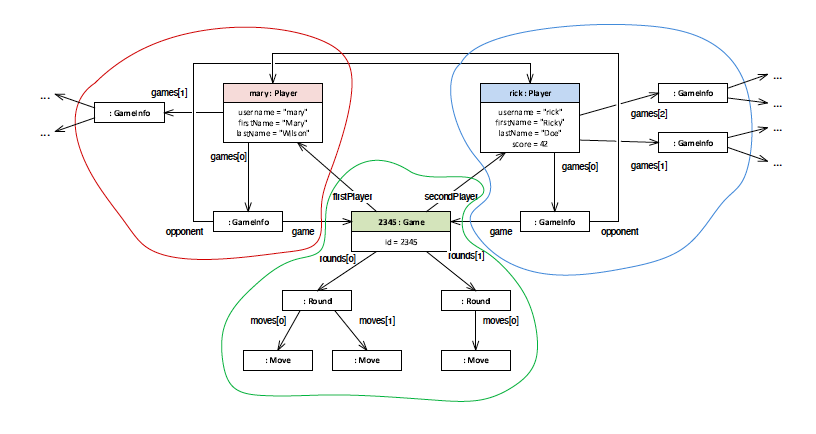
\includegraphics[width=1\textwidth]{img/designAggregati}
Nella figura sopra riportata l'oggetto con lo scomparto superiore colorato é un'entitá, altrimenti
é un oggetto di valore. La linea chiusa denota il confine di un aggregato.
Pertanto avremo due classi aggregate principali: Player e Game.

\subsection{Partizionamento degli Aggregati e modellazione NoSQL}
In questa fase viene utilizzato \emph{NoAM} come modello intermedio tra gli aggregati e i database NoSQL, quindi potrebbe
essere visto come un equivalente della \emph{progettazione concettuale} fatta nei database relazionali.
Il modello NoAM $\to$ modello di dati astratti, ha il compito di sfruttare i punti in comune dei vari modelli di dati, ma
introduce anche astrazioni per bilanciare le variazioni che vi sono tra diversi modelli di NoSQL.
Vi sono due nozioni distinte di \emph{unitá} di accesso ai dati:
\begin{itemize}
    \item \texttt{blocco}, unitá di dimensione maggiore, ha massima consistenza
    \item \texttt{entry}, unitá di dimensione minore, che permetto l'accesso ai dati
\end{itemize}
Con riferimento in particolare ai database chiave-valore una \texttt{entry} corrisponde a una coppia chiave-valore, mentre
un \texttt{blocco} corrisponde a un gruppo di coppie chiave-valore correlate tra loro.
Modello generale:
\begin{itemize}
    \item Un \texttt{database} é un insieme di \texttt{collections}. Ogni \texttt{collection} ha un nome distinto\
    \item Una \texttt{collection} é un insieme di \texttt{blocchi}, ogni \texttt{blocco}
    all'interno della \texttt{collection} é identificato da una chiave di blocco, che deve essere univoca
    \item Un \texttt{blocco} é un insieme non vuoto di \texttt{entries}, ogni \texttt{entry} é composta da una coppia
    chiave-valore, la quale é univoca all'interno del blocco, il valore puó essere anche complesso.
\end{itemize}
Per effettuare il passaggio da aggregati a modellazione NoSQL:
\begin{itemize}
    \item Ogni classe di aggregati viene rappresentata da una \texttt{collection}
    \item Ogni singolo aggregato viene rappresentato da un \texttt{blocco}
\end{itemize}
Vi sono due modalitá principali per rappresentare gli aggregati:
\begin{itemize}
    \item \emph{Entry per Aggregate Object (EAO)}: Rappresenta ogni aggregato utilizzando una singola
    \texttt{entry}, la chiave della \texttt{entry} é vuota, il valore contiene l'intero aggregato 
    \item \emph{Entry per Atomic Value (EAV)}: Rappresenta ogni aggregato per mezzo di piú \texttt{entry}, le chiavi
    di ogni \texttt{entry} devono rappresentare il percorso per accedere al valore di un certo componente(quindi possono esserci anche chiavi
    con nomi strutturati a piú livelli), i valori di ogni \texttt{entry} sono atomici
\end{itemize}
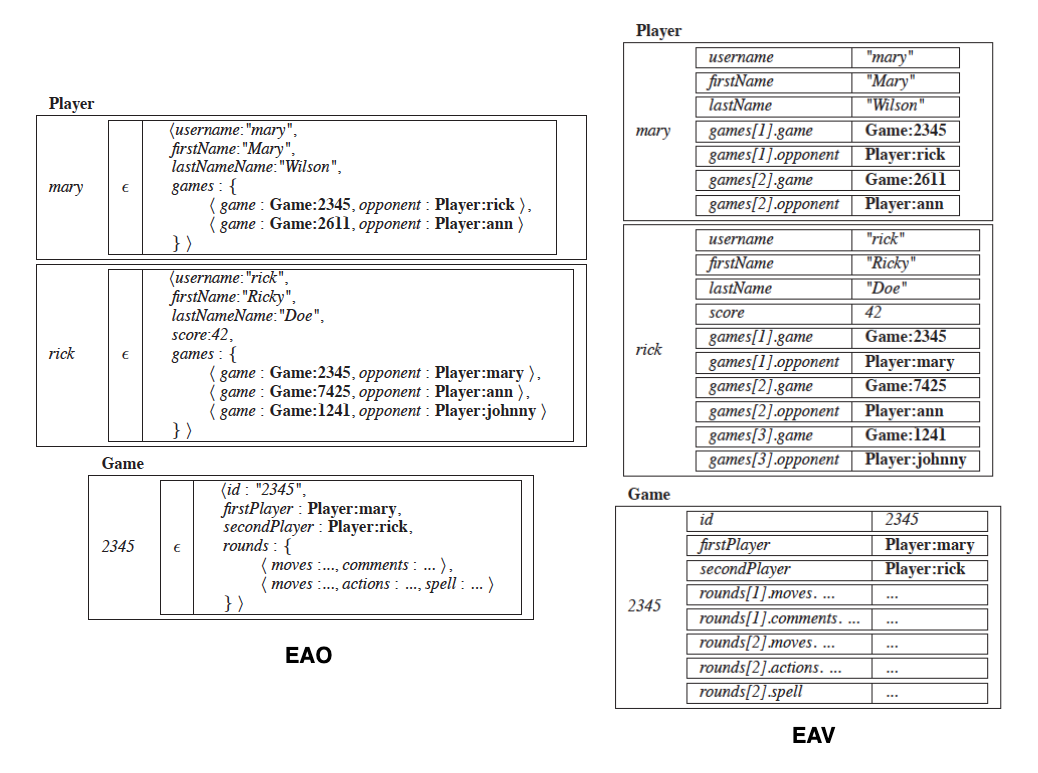
\includegraphics[width=1.15\textwidth]{img/eao:eav}
\\
Nella figura \emph{EAO} si ha per ogni \texttt{blocco} \emph{Player} o \emph{Game} una singola \texttt{entry} con chiave vuota,
valore strutturato in modo complesso \\
Nella figura \emph{EAV} si ha per ogni \texttt{blocco} piú \texttt{entry} in modo da avere valori atomici al suo interno

\subsection{Implementazione}
%continuare...

